\documentclass[11pt,letterpaper]{article}
\usepackage{naaclhlt2015}
\usepackage{times}
\usepackage{latexsym}
\usepackage{url}
\usepackage[pdftex]{graphicx}
\usepackage{breqn}
\usepackage{multirow}
\setlength\titlebox{6.5cm}    % Expanding the titlebox

%%%%%%%%%%%%%%%%%%%%%%%%%%%%%%%%%%%%%%%%%%%%%%%%%%%%%%%%%%%%%%%%%%%%%%
% Code to use with NAACL/ACL style files to simulate natbib's 
% \citealt, which prints citations with no parentheses. This should
% work if pasted into the preamble. \cite, \newcite, and \shortcite
% should continue to work as before.

\makeatletter

\def\citealt{\def\citename##1{{\frenchspacing##1} }\@internalcitec}

\def\@citexc[#1]#2{\if@filesw\immediate\write\@auxout{\string\citation{#2}}\fi
  \def\@citea{}\@citealt{\@for\@citeb:=#2\do
    {\@citea\def\@citea{;\penalty\@m\ }\@ifundefined
       {b@\@citeb}{{\bf ?}\@warning
       {Citation `\@citeb' on page \thepage \space undefined}}%
{\csname b@\@citeb\endcsname}}}{#1}}

\def\@internalcitec{\@ifnextchar [{\@tempswatrue\@citexc}{\@tempswafalse\@citexc[]}}

\def\@citealt#1#2{{#1\if@tempswa, #2\fi}}

\makeatother
%%%%%%%%%%%%%%%%%%%%%%%%%%%%%%%%%%%%%%%%%%%%%%%%%%%%%%%%%%%%%%%%%%%%%%

% Effects of non-linguistic context
\title{Audience and discourse modulate information density on twitter\Thanks{Thanks to...}}
% Information content changes with audience and conversation length in microblog texts
% common ground decreases information

\author{Author 1\\
XYZ Company\\
111 Anywhere Street\\
Mytown, NY 10000, USA\\
{\tt author1@xyz.org}
	  \And
          Author 2\\
ABC University\\
900 Main Street\\
Ourcity, PQ, Canada A1A 1T2\\
{\tt author2@abc.ca}
}

\date{}


\begin{document}
\maketitle
\begin{abstract}
Optimal use of a noisy communication channel requires the uniform distribution of information across a message. The idea that language users might attempt to approximate this kind of optimal usage in their production is known as the ``uniform information density'' (UID) hypothesis. Previous work on UID has suggested that a signature of the hypothesis is an  increase in linguistic information across sentences in a text, presumably compensating for increasing shared context or common ground. We apply the UID hypothesis to data from a popular social media platform and find evidence for differences in information content across different audiences sizes for messages. In addition, we find an unpredicted effect: that information content decreases across small-audience conversations. We interpret these findings in terms of a noisy channel model in which smaller, more responsive audiences allow for message content to be distributed across multiple messages. 


\end{abstract}

\section{Introduction}

Linguistic communication can be viewed through the lens of information theory as communication via a noisy channel.  If humans are approximately rational in their communications and the noisy channel model is appropriate, then we expect to see communication follow an approximately constant rate of information flow.  This is the Uniform Information Density (UID) hypothesis.

Evidence in favor of UID has been found in many levels of language production. At a local level, there is clear evidence from phonology that speakers reduce more predictable sounds \cite{aylett2004,aylett2006,bell2003}, suggesting that they are giving more ``air time'' to less predictable material to equalize information density. And in syntax, speakers tend to drop optional materials (like the word ``that'' as a sentence-complementizer) in more predictable scenarios \cite{levy2007,frank2008,jaeger2010}, again implying a process of allocating communication time relative to predictability. Both of these sets of findings thus suggest at least some local sensitivity to message complexity.

There is also some evidence for UID based on broader considerations, such as linguistic context.  \citealt{genzel2002} showed that word-by-word complexity (measured by a standard n-gram language model) increases across sequences of sentences. They hypothesized that this increase was due to a corresponding increase in non-linguistic information that would make even more complex linguistic structures easier to predict. Follow-ups have shown that this same complexity increase effect is attested in different document types and across languages \cite{genzel2003,qian2012}. 

However, there is an important gap in these tests of the UID hypothesis: little work has been done looking at broad-scale information effects in interpersonal dialogue, the archetype of human linguistic communication.   The contextual studies cited above draw almost exclusively from long, well-structured written texts that function as monologues from writer to reader.  Some studies on phonological and syntactic reduction look at dialogues, but their analysis focuses on local effects, rather than broader context. With the exception of one preliminary study that provided a partial replication of the original complexity increase effect using the Switchboard corpus \cite{vega2009}, to our knowledge no work has explored how the dynamics of conversation interact with UID. 

The present study applies information-theoretic analysis to a corpus of social media microblog posts that include a large number of natural dialogues.  Surprisingly, we do not see clear evidence of the UID hypothesis in these dialogues.  Instead, we propose that a noisy-channel analysis of such dialogues may explain other effects on information content that obscure attempts to attain UID.

\subsection{Conversations, context, and content}

One common motivation for the UID hypothesis is a rational analysis based on a noisy-channel model of communication \cite{levy2007}.\footnote{The other common motivation is a surprisal-based argument \cite{levy2008}: maintaining UID also minimizes the listener's comprehension effort.}  In the noisy-channel analysis, the amount of noise in the channel sets an optimal value for information density to obtain fast, error-free transmission.  For a noise level $\alpha$, we will refer to the optimal information content per discourse unit $Y_i$ as $H_\alpha(Y_i)$.  Discourse units, depending on the analysis, can range from syllables to whole documents; in our analyses, we focus on words and tweets as our discourse units.

In the course of a message, as argued by \newcite{genzel2002}, the actual information content per discourse unit is predicted by the entropy of the random variable $X_i$ representing the precise word choice or choices within the discourse unit, conditioned on the available context.  The precise extent of this context is difficult to pin down. 

We approximate context for our dialogue studies by thinking in terms of the {\it common ground} that a rational speaker believes to exist, given the expected audience of their message. Common ground is defined as the knowledge that participants in a discourse have and that participants know other participants have, including the current conversational context \cite{clark1996}. This common ground can be built from a combination of linguistic and non-linguistic context, including previous messages within the discourse, preceding interactions between the conversation participants, and world knowledge about the topic being discussed.

To formalize this relationship, let $C_i$ be the common ground that exists prior to the production of discourse unit $Y_i$, and let $\alpha$ be the expected noise level in the channel that $Y_i$ is transmitted through.  Then optimality within a noisy channel model predicts that the noise-dependent optimal information rate $H_{\alpha}(Y_i)$ is related to the actual information rate as follows:

\begin{equation}
H_{\alpha}(Y_i|C_i) =  H(X_i) - I(X_i ; C_i) \label{eq:uid}
\end{equation}

Here, $H(X_i)$ is the apparent decontextualized entropy of the discourse unit independent of the common ground.  This quantity is often estimated from a language model that uses only local context, not higher-level discourse context or common ground.  We use a trigram Markov model in this study.

$I(X_i;C_i)$ is the mutual information of the discourse unit random variable $X_i$ and the common ground $C_i$---essentially how much more predictable the next discourse unit becomes from knowing the common ground.  Common ground is difficult to quantify---both in the particular datasets we consider and more generally---so we rely on the assumption that more common ground is correlated with greater mutual information, as in \newcite{genzel2002}.

Then, based on these assumptions, Eq. \ref{eq:uid} allows us to make two UID-based predictions. First, as channel noise increases, transmission error should increase, which in turn should cause the optimal information transfer rate $H_\alpha(Y_i)$ to decrease.  Thus, to maintain equality with rising noise, the apparent entropy $H(X_i)$ should decrease. This prediction translates into communicators ``slowing down'' their speech (albeit in terms of information per word, rather than per unit time) to account for increased errors. 

Second, as common ground increases, $I(X_i;C_i)$ should increase. To maintain equality with rising common ground, $H(X_i)$ should thus also increase, so as not to convey information slower than necessary. This prediction translates into communicators ``going faster'' (e.g., packing more information into each word) because of an assumption that listeners share more common ground with them.

\subsection{The current study}

We take advantage of the conversational structure of the popular social media microblogging platform Twitter (\url{http://twitter.com}) to test these predictions.  Twitter allows users to post 140 character ``tweets'' in a number of different conversational contexts. In particular,  because some tweets are replies to previous tweets, we can use this reply structure to build conversational trees, and to track the number of participants.  In addition, specific choices in tweet production can affect what audience is likely to see the tweet.  These variables are discussed in depth in Section \ref{sect:conversation}.

To test the entropy effects predicted by Eq. \ref{eq:uid}, we first examine different types of tweets that reach different audience sizes.  We then restrict our analysis to reply tweets with varying audience sizes to analyze audience size independently of noise.  Finally, we look at the effects of common ground (by way of conversation structure) on tweet entropy. Contrary to previous UID findings, we do not see a clear increase in apparent entropy estimates due to more extensive common ground, as had been found in previous non-conversational work \cite{genzel2002,qian2012,doyle2015}.  

We propose two factors that may be influencing conversational content in addition to UID factors.  First, considering and adapting to two different types of noise---message loss and message corruption---may cause tweeters to make large-scale decisions that overwhelm any UID effects.  Second, achieving conversational goals may be more dependent on certain discourse units that carry low linguistic informativity but substantial social/conversational importance.

\section{Corpus}

Randomly sampling conversations on a medium like Twitter is a difficult problem. Twitter users routinely use the medium to converse in smaller groups via the \@ mention functionality (described in more detail below). Yet such conversations are not uniformly distributed: A random sample of tweets---perhaps chosen because they contain the word ``the'' or a similarly common token \cite{doyle2014}---does not yield any density of dialogues. Dialogues tend to occur because a user with a sufficient community of followers posts a tweet that causes followers to engage and then responds to at least some of the followers' reactions. 

\subsection{Seed strategy}

To sample such interactions, we developed a ``seed'' strategy where we identified popular twitter accounts and then downloaded a large sample of their tweets, then downloaded a sample of the tweets of all the users they mentioned. This strategy allowed us to reconstruct a relatively dense sample of dialogues (reply chains).

\begin{table}
\begin{center}
\begin{tabular}{|c|c|c|c|}
\hline
Seed Users & Category \\ % & Replies & Non-replies\\
\hline
{\tt @camerondallas} & \multirow{2}{*}{Youtube stars} \\
{\tt @rickypdillon} & \\
\hline
{\tt @edsheeran} & \multirow{2}{*}{Musicians} \\
{\tt @yelyahwilliams} & \\
\hline
{\tt @felixsalmon} & \multirow{2}{*}{Journalists} \\
{\tt @tanehisicoates} & \\
\hline
{\tt @jahimes} & \multirow{3}{*}{Politicians} \\
{\tt @jaredpolis} & \\
{\tt @leezeldin} & \\
\hline
{\tt @larrymishel} & \multirow{2}{*}{Economists} \\
{\tt @paulnvandewater} & \\
\hline
{\tt @neiltyson} & \multirow{3}{*}{Scientists} \\
{\tt @profbriancox} & \\
{\tt @richardwiseman} & \\
\hline
\end{tabular}
\end{center}
\caption{\label{tab:seed-users} Seed users for our dataset.}
\end{table}

We began by choosing a set of 14 seed Twitter accounts that spanned a variety of genres, were popular enough to elicit replies, and interacted with other users often enough to build up a community.  The seed users are listed in Table \ref{tab:seed-users}.  

To build conversations, we needed to obtain tweets directed to and from these seed users. For each seed user, we downloaded their last 1500 tweets, extracted all users mentioned within those tweets, and downloaded each of their last 1500 tweets.  To capture tweets that failed to start conversations with the seed users, we also added the last 1000 tweets mentioning each seed user's handle.  Tweets that appeared in multiple communities were removed.  Each reply contains the ID of the tweet it replies to, so we could rebuild conversation trees back to their roots, so long as all of the preceding tweets were made by users in our communities.

\subsection{Conversation structure and visibility}\label{sect:conversation}

Twitter conversations follow a basic tree structure with a unique root node. Each tweet is marked as a reply or not; for replies, the user and tweet IDs of the tweet it replies to is stored. Each tweet can be a reply to at most one other tweet, so a long conversation resembles a linked list with a unique root node. ``Mentions,'' the inclusion of a username in a tweet, are included in tweets by default throughout a conversation unless a tweeter chooses to remove some of them, so tweets deep in a conversation may be primarily composed of mentions rather than new information.  

Mentions also affect tweet visibility.  Tweets whose first character is a mention (whether or not it is a reply) do not show up by default when browsing a user's tweets, unless the browser follows both the tweeter and first-mentioned user.\footnote{This behavior varies slightly depending on what application is used to view Twitter.  On the website, mention-first tweets do not appear in lists and only appear after clicking the 'tweets \& replies' option on a timeline. On the Twitter mobile app, mention-first tweets appear by default on a timeline but still not in lists.}

After some processing described below, our sampling process resulted in 5.5 million tweets, of which 3.3 million were not part of a conversation (not a reply, and received no replies).  Within this data, we found 63,673 conversations that could be traced back to a root tweet, spanning 228,923 total tweets. Unfortunately, Twitter only tracks replies up a tree, so while we know with certainty whether a tweet is a reply (even if it is to a user outside our communities), we do not know with certainty that a tweet has recieved no replies, especially from users outside our communities. If anything, this fact makes our analyses conservative, as they may understate differences between reply and non-reply tweets. The remaining 2 million tweets were replies whose conversations could not be traced back to the root.

\subsection{Information content estimation}

To estimate the information content of a tweet, we first tokenized the tweets using Twokenizer \cite{owoputi2013}. We then removed any number of mentions at the beginning or end of a tweet, as these are usually used to address certain users rather than to convey information themselves. (Tweets that only contained mentions were removed.)  Tweet-medial mentions were retained but masked with the single type {\it [MENTION]} to reduce sparsity. Links were similarly masked as {\it [URL]}. Punctuation and emoji were retained. We then built trigram langauge models using SRILM with default settings and Kneser-Ney discounting.  Types with fewer than 5 tokens were treated as out-of-vocabulary items. 

For each seed user, the training set was the set of all tweets from all other seed users.  This training set provides tweets that are contemporaneous to the test set and cover some of the same topics without containing the same users' tweets.

\section{Analyses}

We describe the results of three sets of analyses looking at the influence of audience size and available context on apparent tweet entropy. The first examines the effect of expected audience size at a coarse level, comparing tweets directed at a small subset of users, all one's followers, or the wider realm of a hashtag.   The second examines the effect of finer differences in known audience size on apparent informativity.  The third moves into conversations and tracks how conversational context and length affect informativity.

[Note: final values of effect sizes and p-values, based on full regression model, will be added tonight. The graphs also need ot be improved]

\subsection{Expected audience size}
\label{sec:expected}

First, we consider three different types of tweets and their expected audience size.  A tweet whose first word is a mention will not appear in most Twitter visualizations unless the reader follows both the tweeter and the first-mentioned user, or is mentioned somewhere in the tweet. (We will refer to these as ``invisible'' tweets as they are invisible to followers by default.)  A tweeter making an initial-mention tweet thus should expect such a tweet to have a relatively limited audience, with a focus on the mentioned users.\footnote{At least some twitter users consciously manipulate audience using these markers: many tweets have an initial period or other punctuation mark to prevent it from being hidden. Some users routinely switch between initial-mention replies and ``dot''-replies in the course of a conversation to change the audience, presumably depending on their estimate of the wider relevance of a remark.}

\begin{table*}
  \begin{tabular}{|c|l|c|}
\hline
Type & Tweet & Per-word entropy \\
\hline
\multirow{3}{*}{invisible\vspace*{-.7em}} & [MENTION] [MENTION] this is so accurate tho & 6.00\\
\cline{2-3}
 & [MENTION] can you come to my high school ? ;3 & 7.61\\
\cline{2-3}
 & \parbox[][6ex][c]{.7\textwidth}{[MENTION] Hi Kerry , Please send us your email address in order to discuss this matter further . Thanks !} & 8.58\\
\hline
\hline
 & post your best puns in the comments of my latest instagram photo : [URL] & 7.44\\
\cline{2-3}
\multirow{2}{*}{baseline}  & \parbox[][6ex][c]{.7\textwidth}{ I wish I could start a blog dedicated to overly broad and sweeping introductory sentences} & 9.98\\
\cline{2-3}
&\parbox[][6ex][c]{.7\textwidth}{ this new year's eve in NYC , keep an eye peeled 4 Sad Michael Stipe . [URL] already found him : [URL]} & 7.17\\
\hline
\hline
 & I will probably be quitting my job when \#GTAV comes out & 7.63\\
\cline{2-3}
\multirow{2}{*}{hashtagged} & \parbox[][6ex][c]{.7\textwidth}{\#UMAlumni what is the number one thing graduating seniors should know ? \#MGoGrad} & 6.80\\
\cline{2-3}
 & \parbox[][6ex][c]{.7\textwidth}{Brilliant interactive infographic : shows cone of uncertainty for \#climatechange [URL] \#howhotwillitget} & 12.1\\
\hline
  \end{tabular}
 \caption{Example tweets.}\label{tab:ex}
\end{table*}


On the other side, a hashtag serves as a tagging or categorization mechanism so that interested users can discover new content. Hashtags are thus often used to expand the potential audience for a tweet by including in the feeds of users tracking that hashtag, regardless of whether they follow the original tweeter, and so a tweeter using a hashtag should expect a larger audience than normal.\footnote{Not all hashtags are intended for categorization; some are used for emphasis or metalinguistic comment (e.g. \#notmyfavoritefridaymeal, \#toomuchinformation). These comments are probably not intended to broaden the tweet's audience. The presence of such hashtags should, if anything, cause our analysis to underestimate variability across audience types.}  Finally, we have baseline tweets which contain neither mentions nor hashtags and whose expected audience size is approximately one's followers.

Intuitively, context is higher for smaller audiences. Context should be highest for the invisible tweets, where the audience is limited and has seen or can access the previous tweets in the conversation.  Context should be lowest for the hashtagged tweets, where the audience is the largest and will likely contain many users who are completely unfamiliar with the tweeter.  If contextualized UID is the driving force affecting information content, then the invisible tweets should have the highest entropy and hashtagged tweets should have the lowest.

\begin{figure}
 \centering 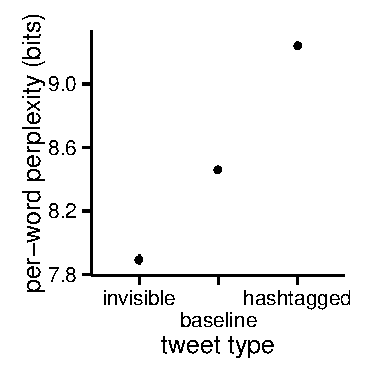
\includegraphics[width=1.7in]{figures/cmcl-audience-pw.pdf}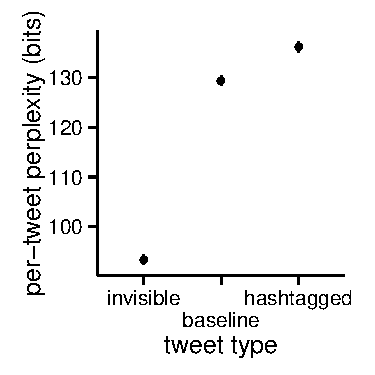
\includegraphics[width=1.7in]{figures/cmcl-audience-pt.pdf}
 \caption{\label{fig:audience} Per-word (left) and per-tweet (right) entropy are higher for tweets with larger expected audience size. By-user 95\% confidence intervals.}
\vspace*{-.5em}
\end{figure}

In this analysis, we use the full 5.5 million tweet database. Figure \ref{fig:audience} plots the entropy of tweets for these three audience sizes.  Per-word and per-tweet entropy both significantly {\it increase} with expected audience size ($p < .001$), the opposite direction of our prediction. We discuss this finding below in the context of our next analyses. 


\subsection{Known audience size}

The results from expected audience size in Section \ref{sec:expected} have a potential explanation (one which points towards our eventual noisy channel account). Different tweet types are accessed are substantially different, and may encourage different kinds of communicative behavior.  Tweets with mentions are highly likely to be seen by the mentioned user (unless the mentioned user is very commonly mentioned), whereas the likelihood of a given hashtagged tweet being seen through the hashtag-searching mechanism is very low.  This uncertainty about audience may lead a rational tweeter to package information into tweets differently: they may include more redundant information across tweets when the likelihood of any given tweet being read is low.

To assess audience size effects in a more controlled setting, we look at tweets with varying numbers of mentions.  Invisible tweets with few mentions have a smaller audience than invisible tweets with more mentions.  Visible tweets, on the other hand, have approximately the same audience size regardless of the number of mentions.  Therefore, we examine the effect of number of mentions in invisible tweets on entropy both in isolation and in comparison to the effect of the number of mentions in visible tweets.  We look only at tweets with at least one mention (as only tweets with mentions can be invisible), and 

\begin{figure}[t]
 \centering
  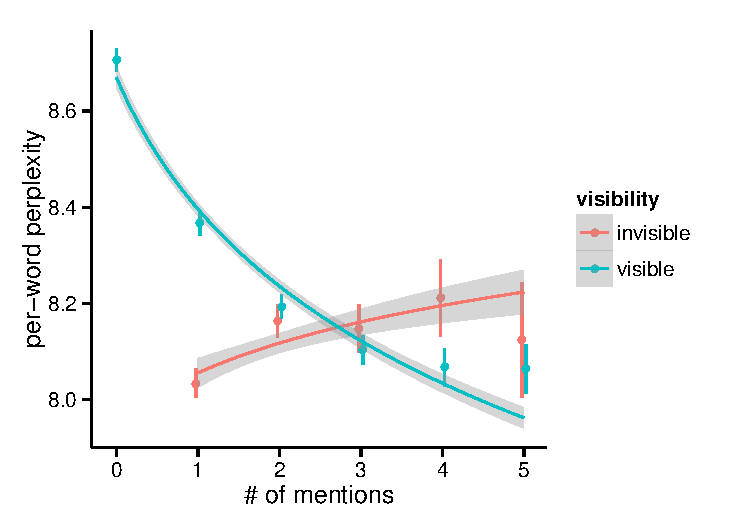
\includegraphics[width=3.25in]{figures/cmcl-mentions-pw2.pdf}
  % 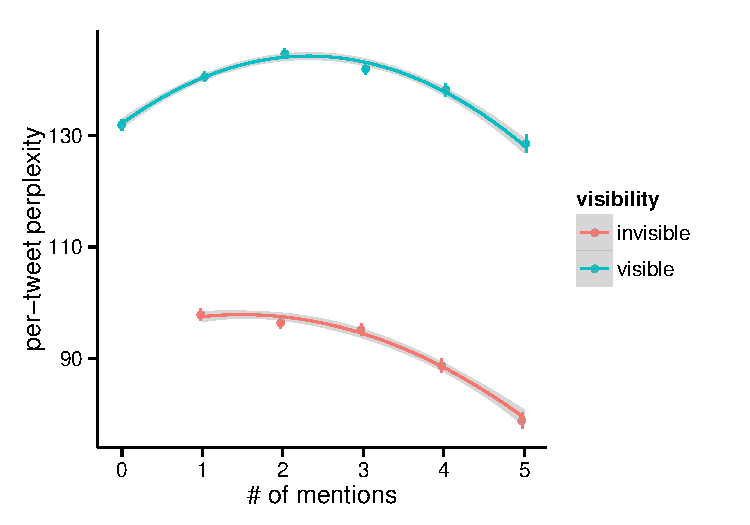
\includegraphics[width=3.25in]{figures/cmcl-mentions-pt.pdf}
 \caption{Per-word entropy of tweets with different numbers of mentions and different visibility.  Invisible tweets' entropy increases with mentions, while visible tweets' entropy decreases.  Logarithmic fits with 95\% confidence intervals.}\label{fig:mentions}\vspace*{-.5em}
\end{figure}

Figure \ref{fig:mentions} shows that the per-word entropy of invisible tweets goes up with the number of mentions, although it levels off as the number of mentions grows.  The per-word entropy of visible tweets goes down with number of mentions.  In both cases, the levelling off is influenced by the increasing number of characters used up by the mentions themselves; with five mentions of usernames of eight characters each (plus space between them and the \@ symbol), this leaves only 90 characters for text.

One possible explanation of this pattern is as follows. For visible tweets, the audience size is relatively independent of the number of mentions, as most tweeters have substantially more followers than the maximum number of mentions in a tweet.  For invisible tweets, the audience size is dominated by the number of mentions, since most of the tweeter's followers are unlikely to see the invisible tweet.  Looking at the interaction between visible and invisible tweet behavior with an increasing number of mentions suggests a controlled effect of audience size.

\subsection{Reply depth and conversation length}

\begin{figure}[t]
 \centering
  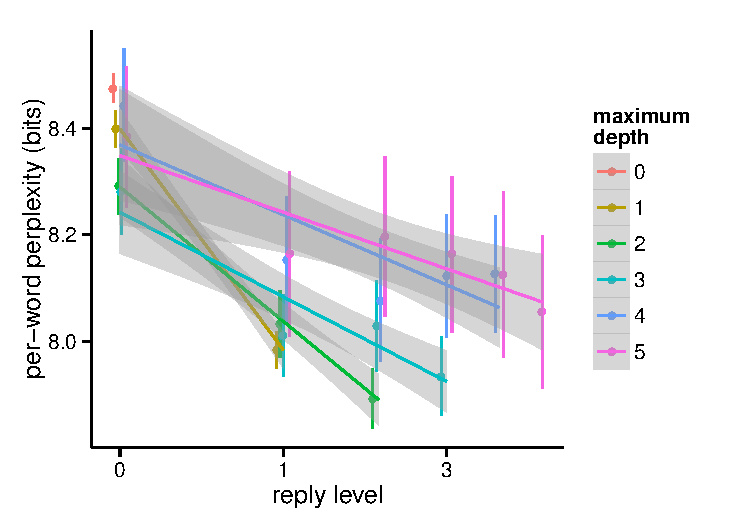
\includegraphics[width=3.25in]{figures/cmcl-rlevel-pw.pdf}
  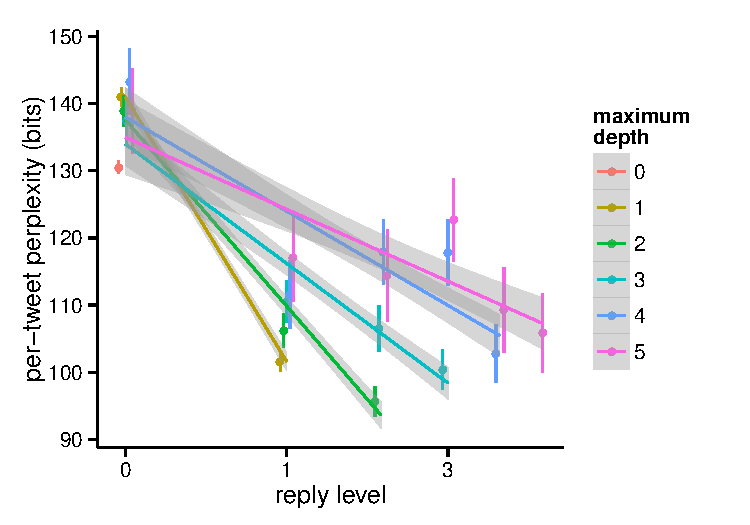
\includegraphics[width=3.25in]{figures/cmcl-rlevel-pt.pdf}
 \caption{Per-word (top) and per-tweet (bottom) entropy decrease with reply level and increase with maximum conversation depth. Linear fits with 95\% confidence intervals.}\label{fig:rlevel-maxdesc}\vspace*{-.5em}
\end{figure}

We next turn to our second UID prediction: that information content should increase as common ground increases. As common ground is assumed to increase in dialogues \cite{clark1996}, we thus predict that twitter conversations should show increases in information content that scale with reply level. Such a result would constitute a replication of \citealt{genzel2002} in the discourse context, and would confirm preliminary results on the Switchboard corpus by \citealt{vega2009}. As is clear from our analysis below, that is not what we found. 

Figure \ref{fig:rlevel-maxdesc} plots mean perplexities for different reply levels and maximum conversation depths, with confidence intervals based on by-user means. Increasing the reply level decreases the information content of the tweet, while increasing the conversation depth increases the information content.

We fit a linear mixed-effects regression model to per-word and per-tweet perplexity.  Control factors were the logarithm of the tweet reply level and the logarithm of the maximum descendant level, along with a separate binary variable for whether the tweet was part of a conversation at all. A random by-user intercept was also included.  Both log reply level and log descendant level had significant effects by likelihood-ratio tests.

Reply level had negative effects on per-word and per-tweet perplexity (per-word: $-.341 \pm .009$; $p < .001, \chi^2(1) = 1466$, per-tweet: $-39.6 \pm .3$; $p < .001, \chi^2(1) =  16777$).

Maximum descendant level had positive effects on per-word and per-tweet perplexity (per-word: $.285 \pm .010$; $p < .001, \chi^2(1) = 817$, per-tweet: $35.1 \pm .3$; $p < .001, \chi^2(1) = 10520$).

Tweets that were not part of a conversation (non-reply tweets that generated no replies) had significantly higher perplexities than non-reply tweets that did generate at least one reply (per-word: $.379 \pm .008$; $p < .001, \chi^2(1) = 2035$, per-tweet: $29.4 \pm .3$; $p < .001, \chi^2(1) = 10372$).  

To summarize these effects, all conversations become more predictable as they go along. The longer the conversation goes, the less predictable it was to begin with, but the most unpredictable tweets fail to start a conversation at all. We discuss these results below.

\section{General Discussion}

Uniform Information Density (UID) is the hypothesis that rational communicators should adjust their messages so as to spread information as uniformly as possible across a message. But do real human communicators actually conform to this expectation? Previous evidences supports this hypothesis in written communications \cite{genzel2002,qian2012} and in some specifics of speakers' phonological \cite{aylett2004} and syntactic choices \cite{levy2007}. 

Our current work synthesizes these two bodies of work by looking for evidence of UID effects in a large corpus of Twitter conversations, including dialogues and broader conversations.  Contrary to expectations, we failed to find UID effects; in fact, we often found information rate \emph{increasing} when context changes would have predicted decreasing information rates.  Specifically, we found that messages to smaller audiences, which should have lower noise and greater context and hence higher information density, actually have \emph{lower} information density than messages to larger, noisier, and less context-sharing audiences. Furthermore, we found that later messages within a reply chain, which should have greater context, also have less information.  This last result is especially surprising because UID context effects have been repeatedly found in more monologous texts.

So should we give up on UID? While our results were unexpected, as we discuss below, we believe that they can be explained with respect to aspects of the Twitter medium and perhaps eventually subsumed into a modified version of the UID theory.

\subsection{Explaining information decreases}

Why do Twitter conversations look different from the increasingly-informative texts studied in previous work? For one, our dataset contains true conversations (dialogues as well as multi-participant exchanges), whereas almost all of the sentence-level context informativity results were based on single-author texts.  Dialogues are often reactive; for instance, a reply may be a clarification question, 
%(EXAMPLES)
which would typically be shorter and more predictable than the original statement. 
Single-author texts are unlikely to include such predictable reactions.

Furthermore, in most of the previously-studied genres, the authors of the texts could reasonably expect their readers to be both focused and unlikely to disengage from reading. Tweets, however, are often read and responded to while doing other tasks, reducing focus and increasing disengagement rates.  Interestingly, the one genre where \newcite{genzel2003} found a negative effect of sentence number on informativity was tabloid newspapers, whose authors can assume that their readers are likely to be distracted and to disengage prematurely.

Both of these factors---a need for discourse maintenance and an audience with limited attention---should mitigate \emph{increases} in information density. But common ground should never \emph{decrease} over the course of a conversation, even on social media, and the ability to look back at previous statements within a written conversation should make common ground more stable as well. Even given these mitigating circumstances, decontextualized estimates of entropy should still increase as shared context increases given the original noisy-channel derivation of UID. We consider two further possible explanations for decreases. 

\subsubsection{Noise as loss of attention}

Perhaps the noisy-channel model should be tweaked for settings such as Twitter. Perhaps the locus of the noise in tweets should not be in comprehension of the tweet per se (or at least not exclusively on comprehension). Instead, perhaps the main source of noise for Twitter users is whether a reader engages with the tweet at all. Many Twitter users follow an enormous number of users, so outside of directed mentions and replies, there is a substantial chance that any given tweet will go unread by the larger part of its intended audience.\footnote{As a result, tweeters often create tweets that include their own context; for instance, a reply may quote part of its preceding tweet, or a user may talk about a recent event and include a link to an article.} 

So the decreases we observed may have to do with users optimizing the amount of information content relative to the likelihood of an audience-member seeing more than one message. For tweets that go the largest audience, this chance is the highest; thus it makes very little sense to spread content over multiple tweets, since a large proportion of the audience will see only one. In contrast, for tweets that are targeted by a mention, it is likely that further clarifications will be read by the intended audience. 

\subsubsection{Social/pragmatic functions of low entropy messages}

Second, perhaps the conversational setting does lead to different, more social uses of language. Previous work on UID in discourse has made use of monologic texts (often from journalistic or factual sources) \cite{genzel2002,genzel2003,qian2012}. These texts are purely designed for conveying information, with no need for social maintenance. In contrast, turn-taking during conversation serves many different purposes \cite{clark1996}, and a short response can be relatively uninformative in pure information theoretic terms while being pragmatically essential. For instance, suppose two tweeters are in an argument and one asks the other a yes/no question.  Due to this context, it is highly predictable that the next tweet will be ``yes'' or ``no'', making the mutual information term of Eq. \ref{eq:uid} very high.  However, the pragmatic information conveyed by either of these one-word answers is very high, essentially containing all the info from the previous question plus a little more.

A related possibility is that conversation relies heavily on meta-linguistic information.  The last tweet in a Twitter conversation, for instance, often looks distinct from the previous tweets; often it is just a single word (e.g., {\it haha}) or an emoji/emoticon.  Similarly, in real life conversations, the last few messages are often goodbyes and other socially-constrained messages.  These are highly predictable, and have low information content whether estimated in or out-of-context.  However, they convey important meta-linguistic information (e.g., acknowledgment, approval), and simply omitting this or replacing it with a response that looks more like its predecessors is clearly sub-optimal behavior for a normal conversationalist.
corpora.


\subsection{Conclusions}


Each of these proposals makes different predictions about conversational behavior.  If the difference between Twitter conversations and other texts is really a matter of different loci for the noise effects, then other dialogue corpora should behave the same as previous monologue corpora.  If, however, our results stem from a core difference between monologues and dialogues, then we would see dialogue corpora continuing to pattern differntly from monologue 

We tested the Uniform Information Density hypothesis, which has been robustly demonstrated in monologue-like settings, on dialogues in Twitter. Surprisingly, we failed to find the predicted effects of context within these dialogues, and at times found evidence for effects going in the opposite direction.  We proposed possible explanations for these unexpected effects, which will require further experimentation to fully assess.

%\section*{Acknowledgments}
%
%We gratefully acknowledge the support of ONR Grant N00014-13-1-0287.

\newpage
\bibliographystyle{naaclhlt2015}
\bibliography{tweetdiscourse}

\end{document}